\chapter{Implementation}
\label{cha:implementation}

Of course there are multiple ways on how to implement our desired application, so we first take a look on what kind of technology is even available.

\section{Available Hardware}
There are currently multiple AR devices on the market, with many of them being some sort of glasses but with the increasing power of smartphones, AR applications also became available for them. That may be the easiest and widely available form. There are even concepts for motorcycle helmets with integrated displays to give the driver real time information while on the road~\cite{jarvish}. \newline 
One of the better known head-mounted device is the Microsoft HoloLens~\cite{hololens} which runs a Windows operating system (OS) and is therefore relatively easy to use. That is also the reason why we used it in our solution. Another device that attracted some attention a few years ago is the Google Glass~\cite{googleglass} which is, compared to the HoloLens, much lighter and smaller. But also AR on smartphones is, thanks to ever rising performance, wide spread. One powerful application for it is e.g. Google Lens~\cite{googlelens}.


\section{Available Software}
Every device has, depending on the vendor, a different OS and therefore also different applications that can be used. For example, the Google Glass uses Glass OS which is based on Android and also has an API for developers to make their own apps. The HoloLens on the other hand, uses the Windows Mixed Reality platform which is part of Windows 10. That means it can run Universal Windows Platform apps that can be loaded directly from the Windows store and has a Holographic API for 3D applications.


\section{Features}
Most of the available AR glasses have some integrated features that enhance the usability of the device. How good they work of course depends on the vendor. Many have an integrated camera, either to just take photos/videos or, like it is the case with the HoloLens, to track the room and hand movements for controlling. Another feature that can be used for that is eye tracking. For that the device needs a camera on the inside, which unfortunately makes it even bigger. Gesture input is another common technique to interact with the device.


\section{Used Technologies}

For realizing our project, we picked a wide range of both soft- and hardware.

\subsection{Software}

\begin{description}
	\item[LDraw]
	
	LDraw~\cite{ldraw} is a collection of software tools to model LEGO designs, created by James Jessiman. Today it is maintained and further developed by the community. From this tool collection we just use the file formats .ldr and .mpd (Multi-Part Document) and the large library of parts for the models. The .ldr file tells us all the steps and which bricks are used in this phase. Additionally to the file name of the new brick, it also tells us the color and orientation in space. In the brick files we have information about lines, triangles, quads, and in most of them also references to other files, so that common structures do not have to be defined in every file but can be shared. For parsing that means we can work with recursion. There is also much more additional information in these files, which we mostly ignore since it is irrelevant to us.
	
	\item[Python]
	
	For the preprocessing of the model step files we used Python 3.8.1~\cite{python}, an easy and powerful scripting language. We use it to read the .ldr or .mpd model files and translate them to meshes that we save in .obj files to later load the model in Unity. 
	
	\item[Wavefront OBJ/MTL]
	
	This file format is used for the step models, since Unity can easily read and understand it without the need for us to write our own parser. It is one way to describe 3D meshes. The files are saved in plain text so humans can read it. To describe a model, the file first specifies vertices and then faces that reference them. Additionally, it is also possible to define vertex normals and texture coordinates. Since the LDraw format does not provide textures but only the colors of the bricks, we are also using the material template library (.mtl) to specify the colors/materials of the objects.
	
	\item[Unity/C\#]
	
	Unity~\cite{unity} is an application for creating games and applications. We use it to build our program for the HoloLens, where we load our generated .obj files for each step and show them to the user. C\# is the language used in Unity to write additional scripts.
	
	\item[Mixed Reality Toolkit for Unity (MRTK)]
	
	This toolkit~\cite{mrtk} is a Unity framework, developed and distributed by Microsoft, and is especially designed for use with the HoloLens, also distributed by the same company. It provides many useful functions and scripts for building and interacting with apps in AR.
	
	\newpage
	\item[Windows]
	Since we are using the HoloLens, which runs a Windows OS, we decided it would also be best to use a Windows PC to code and build our Unity application. Also the preprocessing which is done with Python was coded on Windows even though it also runs on Linux.
	
\end{description}

\subsection{Hardware}

\begin{description}
	\item[HoloLens 1]
	
	The HoloLens is one of the available 3D AR glasses and is developed by Microsoft. Currently the 2nd version is available but for our project we used the 1st generation. It uses a common, popular OS, Windows, which has many good maintained tools to develop applications for it.
\end{description}

\section{Application}

The goal of the project is to create an application for the HoloLens that gives the user instructions for building a LEGO model step by step. The app should let the user select a model and display the bricks for each step in Augmented Reality on the glasses.
For that we use a two step approach. First we preprocess the input files and then build and compile our Unity app that uses the created model files. The plan is to use the instructions from the input file, that we got from the LDraw Model Repository~\cite{omr}. Most of the models from there have information about the bricks that we need per step. As a backup, in case there are no instructions, we just create a step for every brick.

\subsection{Step 1: Preparing the Model}

To show the model step after step, we first have to parse the given model file. We are working with the open source model description file format LDraw, which provides us with .ldr files. These describe lines, triangles and quads. The problem is that Unity, the application we will use to display the models, does not understand this file format. Therefore we are using the Python scripting language to read the .ldr files and write out a model in the Wavefront OBJ file format for each step. Additionally we are writing a file for the whole model. To represent the color of the models, the Material Template Library format (.mtl), a companion file format to .obj, is used.

\subsubsection{Input}
We have two options on how to describe our input. The Multi-Part Document (.mpd) and the LDraw (.ldr) file format. Our parser works with both of them and can create a valid set of input files for the second step.

\begin{description}
	\item[MPD]
	The Multi-Part Document is a file that comes from the Official Model Repository (OMR)~\cite{omr} and describes a brick set, released by LEGO. It has a standardized file name with information about the set name and number and in principle just contains one or multiple models in the .ldr format. They in return refer to multiple .dat files that describe the bricks.
	
	\item[LDR]
	The LDraw file describes the orientation and coordinates of multiple bricks of a model in 3D space. It consists of multiple lines, each one starting with an integer that describes the kind of line. There are 6 different line types: 
	\begin{enumerate}
		\item[0] Commands or META command like information about new steps.
		\item[1] Sub-file reference and their orientation and coordinates.
		\item[2] Line between two points, typically edges of bricks.
		\item[3] Filled triangle between three points.
		\item[4] Filled quadrilateral between four points, defined in either clockwise or counter-clockwise winding order.
		\item[5] Optional line between two points, that is only shown from an certain perspective.
	\end{enumerate}
	All types, apart from 0, contain at least the 3D coordinates (X,Y,Z) of one point, all of them also contain an integer that describes the color of the item. This color has to be looked up in a dictionary because the number says nothing about the red-green-blue (RGB) values. Line type 1 defines a homogeneous transformation matrix, with which we have to multiply all points in the referenced file.\newline
	We do not parse line type 5, since it only represents optional lines that are shown depending on the perspective. We do not care about them, we only want the minimum so we can still understand the model but do not have any unnecessary overhead.
	
\end{description}

\subsubsection{Output}
As output we get multiple files that we will need in the second step. Most of them are Wavefront Object files (.obj file ending), additionally we also create one normal text file (.txt) that contains the name of all available models and a file with the colors. We get the following 3 files, some of them can also occur more often, depending on how many steps or bricks we have.
\begin{description}
	\item[Steps]
	The most important thing we want to extract from our .ldr file is a model of every step. For that we used the .obj file format which contains our vertices and surfaces between them. The more steps we have, the more of these files we get.
	\item[Colors]
	To give the models the same color as in the .ldr files, we have to use the .mtl file format, so for every model we parse, we create one color.mtl file. Since it contains a dictionary of the LDraw colors (every color number is represented as a material), we just need to write one for all step models.
	\item[Small models]
	For showing the small model at the side, we write an extra .obj, which contains all the step files copied together, so we get the final model mesh. That is not the optimal solution, since we also create points and triangles, that are not seen inside of the finished model but it is simple and fast in creation. Also many points get defined multiple times, even if they are used from various items.
	
\end{description}


\subsubsection{Preprocessing}

As mentioned earlier, we decided to use Python for preparing the model. It is very simple to read and write files with it and is also object-oriented, a feature we can use to our advantage, after all we are dealing with multiple bricks. 
We create our own brick class that has all features that we get from our input: color, position, orientation and file name. Additionally, every brick object also has lists of all its lines, triangles, quads and eventually sub-bricks. These things are again represented with their own classes. 

\subsubsection{Build Assets}
For the second step, we have to prepare our models and build asset bundles. To do that, we have to write a build script that can later be started in the Unity editor. Unfortunately we can not build them directly without opening the editor since we have to manually add our meshes to the respective packages. In our script, that has to be in the folder \verb|Assets/Editor/| of our Unity project, we define the output path and with \verb|BuildAssetBundles(string| \verb|outputPath, BuildAssetBundleOptions assetBundleOptions,| \newline
\verb|BuildTarget targetPlatform)| we build our asset bundles for the \newline \verb|targetPlatform|, in our case \verb|BuildTarget.WSAPlayer| since applications on the HoloLens are Windows Store Apps.

\subsection{Step 2: Unity App}

In the second step, we want to build an application for the HoloLens, where we can pick a model to be shown step by step. To do so, we used Unity to make and build the app and Visual Studio to debug it while running on both the HoloLens emulator and the actual AR device.  \newline
The app structure is simple, it has just one scene with an interface for picking the model. For that there is a drop down menu that gets filled at run-time with all models we have. This information is in the file \verb|models.txt| which gets updated every time we prepare a new model with our Python script. Additionally, there is some text for the user, as we can see in Figure~\ref{fig:model_picker}. \newline 
After picking the model, this interface disappears and the first step of the picked instruction gets shown. Furthermore, a small preview of the finished model appears in the upper right corner. Both these meshes get loaded at run-time, depending on which instruction the user picks. In the background, the app loads all of the steps in advance and sets all step meshes up to the current visible and all others invisible.

\begin{figure}[!ht]
	\captionsetup{justification=centering}
	\centering
	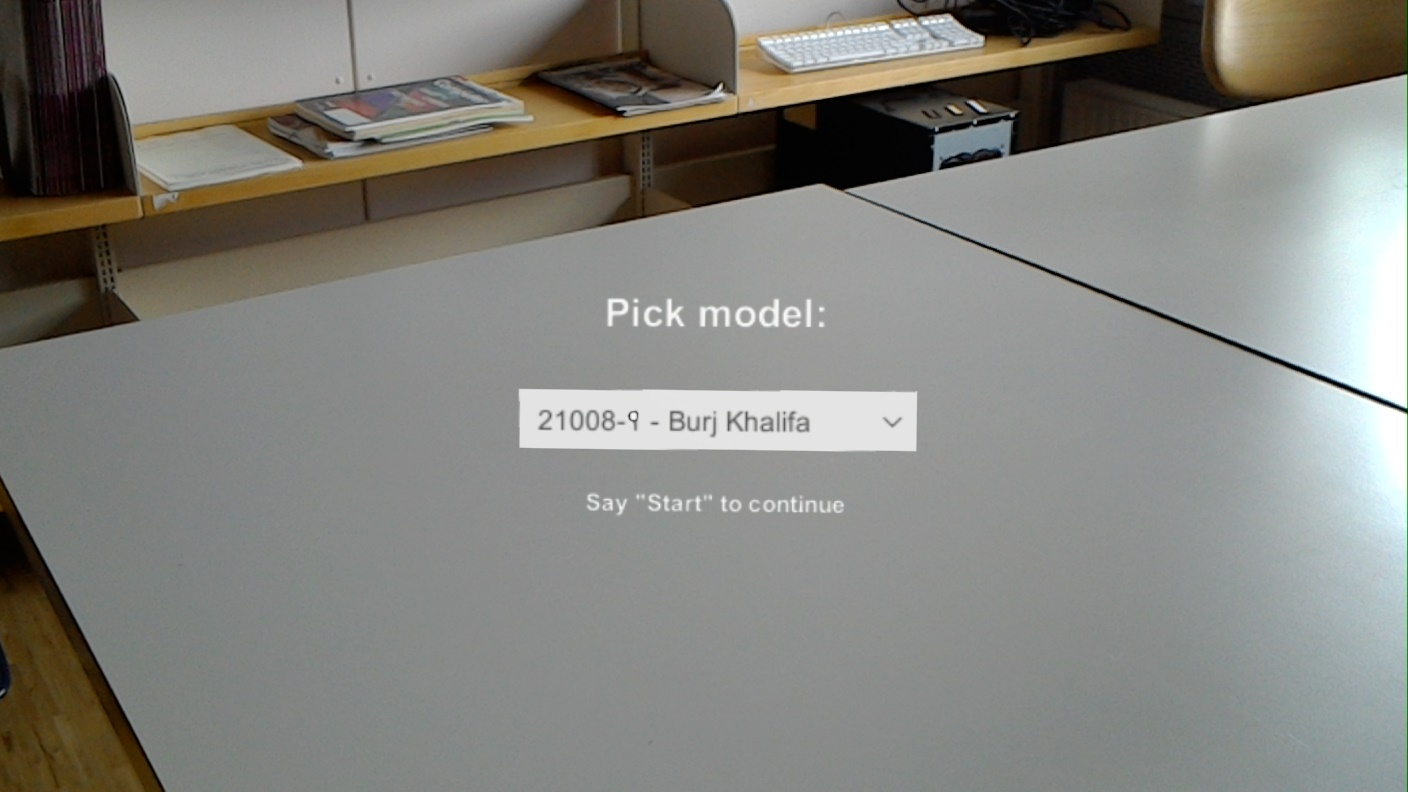
\includegraphics[width=0.9\textwidth]{media/model_picker.jpg}
	\hfill
	\caption{Start screen.}
	\label{fig:model_picker}
\end{figure}

\subsubsection{Voice Commands}
For controlling our instructions, we wanted to use voice commands. For this, we made use of the MRTK Voice Input. We first had to define our keywords and then add a response to these words later on. Since we load our model at runtime, we also want to add the responses later on in our C\# script.\newline 
Only two of the keywords could be added in advance, the one to start our picked model in the beginning and the one for going back to the model selector. The ``Start'' keyword is the only one we need at the menu screen and it gets disabled once the model is picked. In Table~\ref{tab:keywords} we can see our available words and the information what they trigger and when they are added. We decided to add even more keywords than what was planned in the beginning to make the model handling easier.

\begin{table}[thb]
	\centering
	\begin{tabularx}{\linewidth}{|c|L|c|}
		\hline
		\textbf{Keyword} & \textbf{Response} & \textbf{Added at runtime} \\ \hline
		Start & Starts the instructions for selected model & \\ \hline
		Back & Ends the instructions and goes back to the model picker & \\ \hline
		Next & Shows the next step & X \\ \hline
		Last & Shows the last step & X \\ \hline
		Drop & Enables Gravity so that the model can be placed & X \\ \hline
		Come Back & Brings the model back in the users view and disables gravity & X \\ \hline
	\end{tabularx}
	\caption{Usable keywords to control the application}
	\label{tab:keywords}
\end{table}


\subsubsection{Preview}
On the top right corner we added a small replica of the finished  model. To prevent the user to loose this preview, it is fixed to the camera object. That way, it will always stay in the same place. Unfortunately, that makes it impossible to focus and therefore grab or modify it to have a better look at it from all angles. To solve this, we wrote and added a small C\# script to make it rotate.
This is the very simple code that we used:

\begin{verbatim}
using UnityEngine;
public class RotatingObject : MonoBehaviour
{
  public float xAngle, yAngle, zAngle, speed;
	
  void Update()
  {
      transform.Rotate(xAngle*speed, yAngle*speed, zAngle*speed);
  }
}
\end{verbatim}

We see that we have 4 public variables, x-,y- and z-angle and the speed. The angles can be set to by how many degrees times speed the model should be rotated. They can be changed at runtime from any other script.

\subsubsection{Highlighting} 
Highlighting is an essential point in our application for better recognition of the bricks of the current step. The first approach was to let the bricks of the current step emit light, which turned out to be not that bright. To solve that, we changed it up a little bit and simply change the color of the material. We let it pulse between the original color and very light gray. That helps the user to clearly see which parts are new, while also seeing the original indented color. To every step model we added a script in which we where saving the original colors before we started our application. We have a public boolean that gets set to true if the step is the current one and in the Update() function we check for that variable:
\begin{verbatim}
void Update()
{
  if (activeStep)
  {
    int i = 0;
    foreach (Material mat in materials)
    {
      mat.color = Color.Lerp(startColors[i],
                             Color.white * 0.8f,
                             Mathf.PingPong(Time.time * 0.2f, 1));
      i++;
    }
  }
  else
  {
    int i = 0;
    foreach (Material mat in materials)
    {
      mat.color = startColors[i];
      i++;
    }
  }
}
\end{verbatim}

\verb|Color.Lerp((Color a, Color b, float t)|\footnote{\url{https://docs.unity3d.com/ScriptReference/Color.Lerp.html}} linearly interpolates between the first and second parameter (original color and very light gray) by t, \newline \verb|Mathf.PingPong(float t, float length)|\footnote{\url{https://docs.unity3d.com/ScriptReference/Mathf.PingPong.html}} returns a value that increments and decrements between 0 and length. The first parameter t has to be a self-incrementing one, like the time.\newline
Another possible way would be to change the shader for the current step to one that highlights the edges or changes the color in another way.

\section{Workflow}
Currently, to get an instruction of a model of our choice we have to pursue the following steps:
\begin{enumerate}
	\item
	Start the Python script with following command: \newline
	\verb|python main.py path/to/model/file|.
	
	\item
	Open the project in Unity.
	
	\item
	Navigate to the folder \verb|Assets/Models/name_of_model| and add all the models in that folder to a new asset package with the name of the model at the bottom of the inspector pane.
		
	\item
	Build the app in Unity.
	
	\item
	Open the build project in Visual Studio and deploy it to the HoloLens.
	
	\item
	Start the application on the HoloLens.
\end{enumerate}

%\begin{figure}[!ht]
%	\captionsetup{justification=centering}
%	\centering
%	\subfloat[{Adding to asset bundle.}]{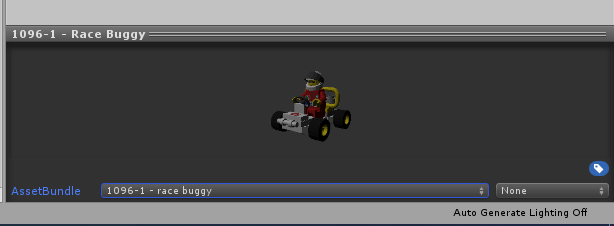
\includegraphics[width=0.47\textwidth]{media/asset_bundle.png}\label{fig:asset_bundle}}
%	\hfill
%	\subfloat[{Bulding asset bundle menu entry.}]{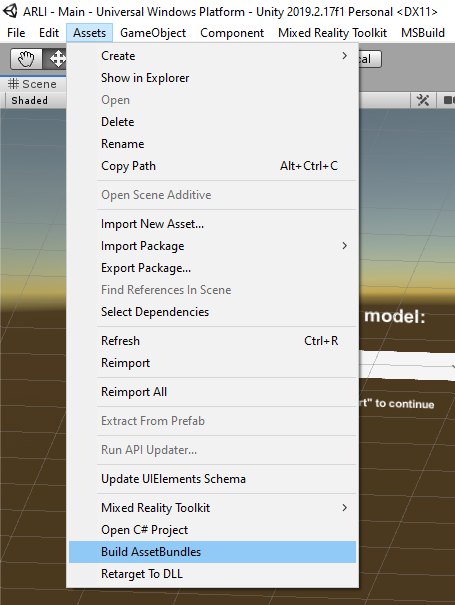
\includegraphics[width=0.47\textwidth]{media/build_asset_bundle.png}\label{fig:build_asset_bundle}}
%	\hfill
%	\caption{Working with asset bundles.}
%	\label{fig:bundles}
%\end{figure}



